\subsection{Avatar animation}
% \dq{Application Center}

{\nameofmethod} empowers controllable avatar animation in various aspects. It enables animating characters using explicit driving signals(e.g., speech signals, expression templates, and pose templates). In addition, it also integrates the implicit driving paradigm using text prompts. Fig. \ref{fig:application-method} shows how we leverage the power of {\nameofmethod} to animate characters from multi-modal conditions. To maintain strict appearance consistency, we modify the {\nameofmethod} architecture by inserting latent of reference image as strong guidance. As shown in Fig. \ref{fig:application-method} (b, c), we encode reference image using 3DVAE obaining $z_{\rm ref} \in \mathbb{R}^{1 \times c \times h \times w}$, where $c = 16$. Then we repeat it $t$ times along temporal dimension and concatenate with $z_t$ in channel dimension to get the modified noise input $\hat{z}_t \in \mathbb{R}^{t \times 2c \times h \times w}$. To achieve controllable animation, various adapters are employed. We describe them in following.

\begin{figure}[h]
    \centering
    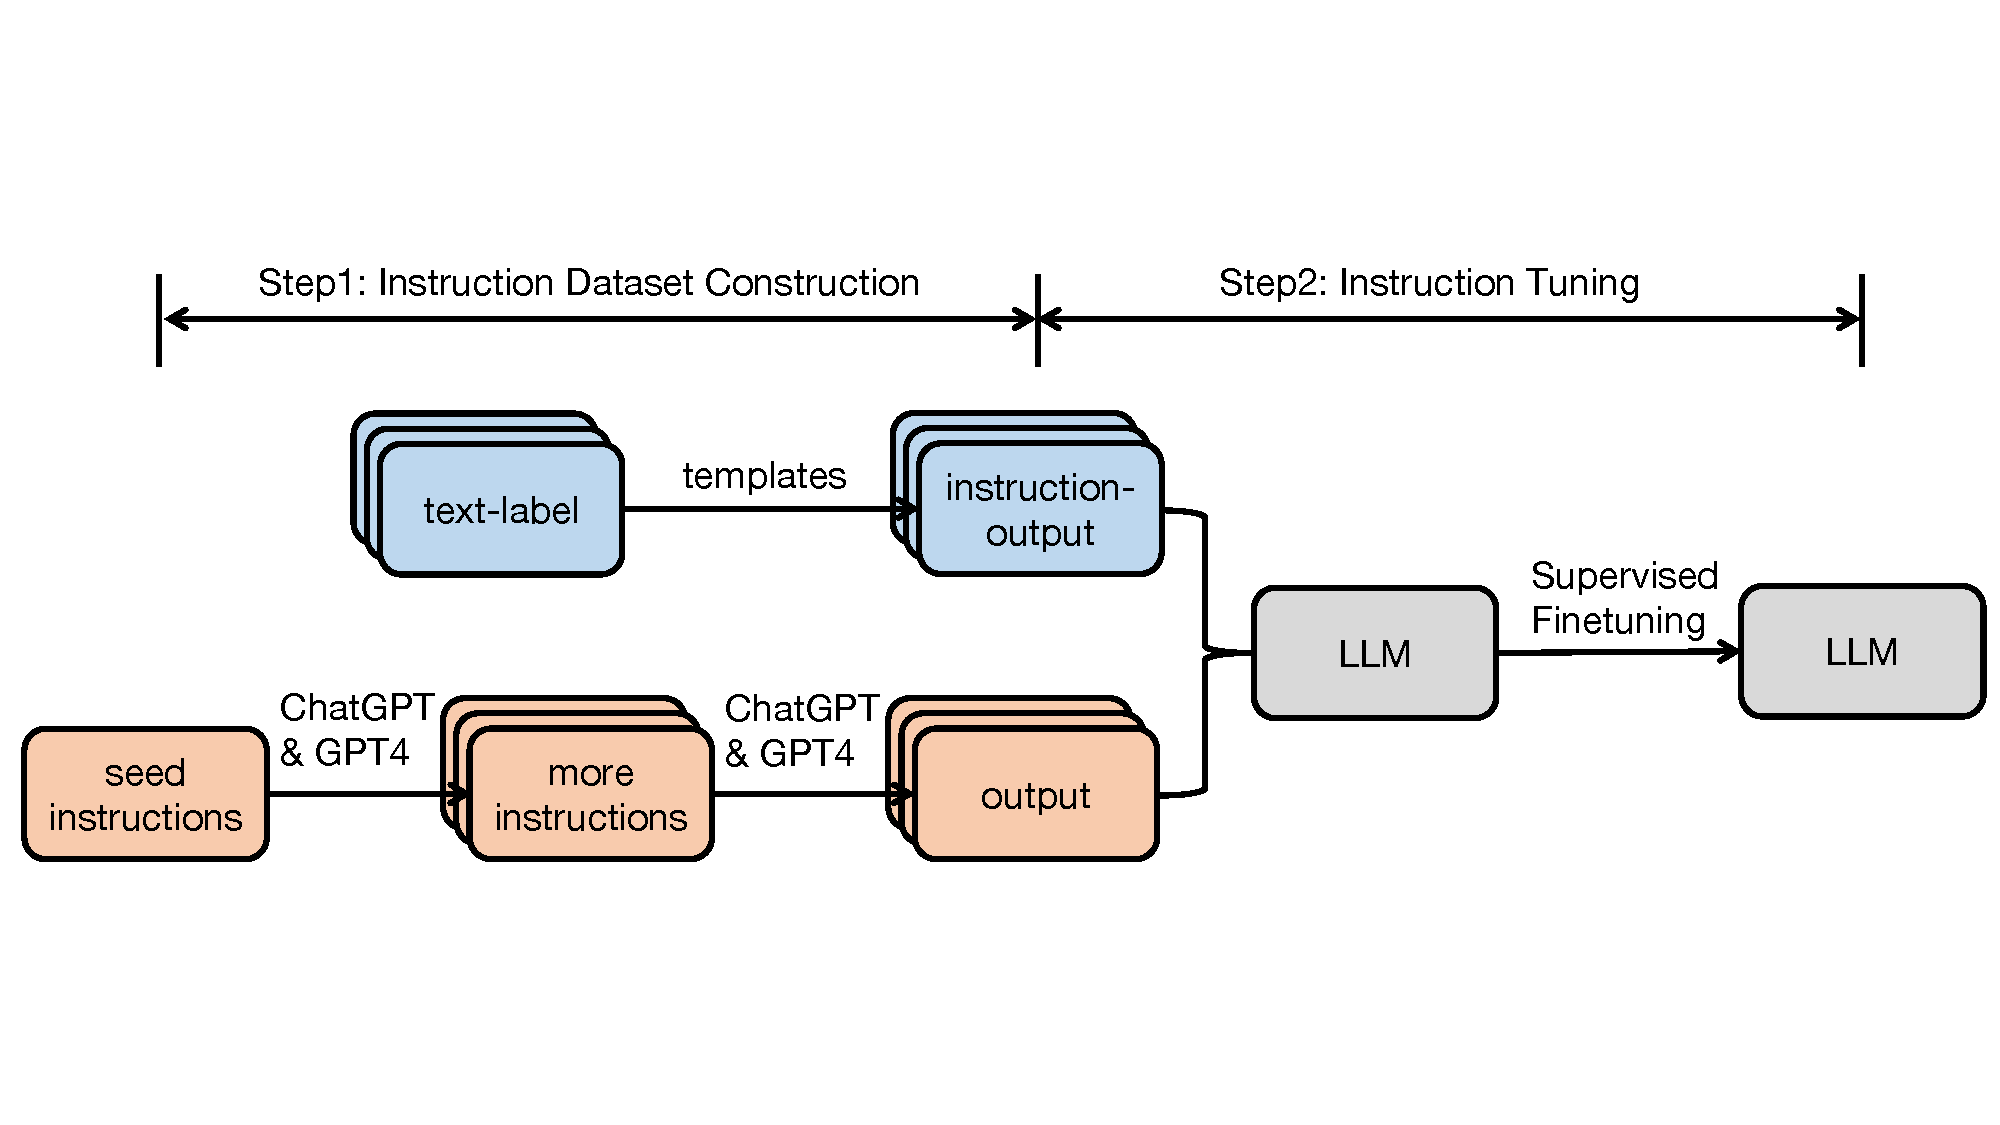
\includegraphics[width=\linewidth]{applications/app_figures/method.pdf}
    \caption{\textbf{Overview of Avatar Animation built on top of \nameofmethod}. We adopt 3D VAE to encode and inject reference and pose condition, and use additional cross-attention layers to inject audio and expression signals. Masks are employed to explicitly guide where they are affecting.}
    \label{fig:application-method}
\end{figure}

\subsubsection{Upper-Body Talking Avatar Generation}

In recent years, audio-driven digital human algorithms have made significant progress, especially in the performance of the talking head. Early algorithms, such as loopy~\cite{ye2024mimic}, emo~\cite{tian2024emo}, and hallo~\cite{xu2024hallo}, mainly focused on the head area, driving the digital human's facial expressions and lip shapes by analyzing audio signals. Even earlier algorithms, like wav2lip~\cite{prajwal2020lip} and DINet~\cite{zhang2023dinet}, concentrated on modifying the mouth region in the input video to achieve lip shape consistency with the audio. However, these algorithms are usually limited to the head area, neglecting other parts of the body. To achieve a more natural and vivid digital human performance, we propose an audio-driven algorithm extended to the upper body. In this algorithm, the digital human not only synchronizes facial expressions and lip shapes with the audio while speaking but also moves the body rhythmically with the audio.

% \subsubsection{Audio-Driven}
\paragraph{Audio-Driven}
Based on the input audio signal, our model can adaptively predict the digital human's facial expressions and posture action information . This allows the driven character to speak with emotion and expression, enhancing the digital human's expressiveness and realism. 
As shown in  Fig. \ref{fig:application-method} (b), for the single audio signal-driven part, the audio passes through the whisper feature extraction module to obtain audio features, which are then injected into the main network in a cross-attention manner. It should be noted that the injection process will be multiplied by the face-mask to control the audio's effect area. While enhancing the head and shoulder control ability, it will also greatly reduce the probability of body deformation. To obtain more lively head movements, head pose motion parameters and expression motion parameters are introduced and added to the time step in an embedding manner. During training, the head motion parameters are given by the variance of the nose tip keypoint sequence, and the expression parameters are given by the variance of the facial keypoints. 
% During inference, fixed values pose=8 and exp=16 are used for inference.
% However, since there is no strong semantic correlation between audio itself and gestures, for some scenes, single audio-driven may cause the head and shoulder part to move naturally with the audio, but the body part, especially the hands,  tends to move slightly or unnaturally. To solve this problem, we introduce text information.


% \subsubsection{Audio and Text Driven}
% \paragraph{Audio and Text Driven}
% Based on aries' powerful semantic understanding ability, we inject a prompt describing actions as the model's text information. In this way, during video generation, the model can not only use audio signals to drive the digital human's actions but also refer to text information to provide more accurate and natural action information. 

% Unlike audio-driven, when we jointly drive with audio and text, we remove the face-mask, allowing the audio's effect area to be released and enabling the character to have a larger range of motion. Second, we removed the encoding of reference images based on llava. During audio-driven, without text injection, we use reference images for information injection. When there is text information, we prioritize aligning with the model's original input. Additionally, we retain the head pose motion parameters and expression parameters.

% By combining audio and text information, our algorithm can achieve a more natural and lively digital human performance. This method not only improves the realism of the digital human but also enhances its adaptability and expressiveness in different scenarios. 


\begin{figure}
    \centering
    \ifhq
    
\includegraphics[width=\linewidth]{hqapplications/audio.png}
    \else
    \includegraphics[width=\linewidth]{applications/app_figures/audio-1.pdf}
    \fi
    \caption{\textbf{Audio-Driven}. {\nameofmethod} can generate vivid talking avatar videos.}
    \label{fig:application-audio}
\end{figure}

\begin{figure}
    \centering
    \ifhq
    \includegraphics[width=\linewidth]{hqapplications/pose.png}
    \else
    \includegraphics[width=\linewidth]{applications/app_figures/pose.pdf}
    \fi
    \caption{\textbf{Pose-Driven}. {\nameofmethod} can animate wide variety of characters with high quality and appearance consistency under various poses.}
    \label{fig:application-pose}
\end{figure}


\begin{figure}
    \centering
    \ifhq
    \includegraphics[width=\linewidth]{hqapplications/expr.png}
    \else
    \includegraphics[width=\linewidth]{applications/app_figures/expr-1.pdf}
    \fi
    \caption{\textbf{Expression-Driven}. {\nameofmethod} can accurately control facial movements of wide-variety of avatar styles.}
    \label{fig:application-expr}
\end{figure}

\begin{figure}[h]
    \centering
    \ifhq
    \includegraphics[width=\linewidth]{hqapplications/pose-expr.png}
    \else
    \includegraphics[width=\linewidth]{applications/app_figures/pose-expr-1.pdf}
    \fi
    \caption{\textbf{Hybrid Condition-Driven}. {\nameofmethod} supports full control with multiple driving sources across various avatar characters.}
    \label{fig:application-pose-expr}
\end{figure}